\documentclass[12pt]{exam}
\pagestyle{headandfoot}
\firstpageheader{}{}{}
\runningheader{\date}{}{\class, \teacher}
\runningheadrule
\firstpagefooter{}{}{}
\runningfooter{}{Viel Erfolg!}{Seite \thepage\:von \numpages}
\runningfootrule
%=========================================================
\newcommand{\theme}{Trigonometrie}
\newcommand{\teacher}{Jonas Guler}
\newcommand{\class}{2GaMa}
\newcommand{\serie}{Repetitionsprüfung}
%\newcommand{\date}{\today}
\newcommand{\duration}{45 Minuten}
\newcommand{\name}{\bf Name:}
\newcommand{\grade}{Note:}
\newcommand{\datum}{26.02.24}
%=========================================================
\begin{document}
\fontsize{14}{14}\selectfont
%========================================================

%========================================================
\begin{tabular*}{\textwidth}{l @{\extracolsep{55mm}}l @{\extracolsep{6pt}}l}
    \textbf{\theme} & \textbf{\grade} & {\answerbox}\\
    \textbf{Klasse \class} & & \\
    \textbf{\teacher}  & {\name} &\textbf{\hrulefill}\\[8pt]
\end{tabular*}
%--------------------
\begin{center}
\rule[1ex]{\textwidth}{1pt}
Dauer: \duration \hspace{9cm}Datum: \datum\\
\vspace{5pt}
\rule[2ex]{\textwidth}{1pt}
\end{center}
%=========================================================

%=========================================================
\begin{center}
\textbf{Bewertungstabelle}\\
\small Wird von der Lehrperson ausgefüllt\\
\vspace{5pt}
\addpoints
\gradetable[h][questions]\\
\vspace{5pt}
Der Rechenweg muss \textbf{vollständig und nachvollziehbar} sein.\\
Lösen Sie die Prüfung mit einen schwarzen oder blauen Kugelschreiber. Resultate in Bleistift, roter oder grüner Farbe werden nicht berücksichtigt.\\
Die Schlussresultate sind vollständig gekürzt oder auf drei Nachkommastellen genau anzugeben.\\
Als Hilfsmittel ist ein Tascherechner erlaubt. Kennzeichne in deinem Lösungsweg klar, wo du den Taschenrechner zur Hilfe genommen hast.
\end{center}

\noindent
\rule[1ex]{\textwidth}{1pt}

\vfill
\begin{center}
    %\Huge{\serie}
\end{center}

\newpage
\begin{questions}
%=========================================================
%-------------------TESTFRAGEN
%=========================================================
\question[3] % Geo2 S38 A18a
Berechne den Inhalt der eingefärbten Fläche. $M$ ist dabei der Mittelpunkt des Kreisbogens.
\begin{figure}[ht]
    \centering
\includegraphics[scale=0.7]{Trigonometrie/data-trigo/Sektorfläche.png}
\end{figure}
\vspace{5pt}
\antwort{16}


%---------------------------------------------------------
\newpage
\question[5] % Funktionsgraphen
\textbf{Beachte:} Lösungswege mit Hilfe des Taschenrechners gibt keine Punkte!
\begin{parts} 
    \part Zeichne den Winkel $\alpha=165^\circ$ im Einheitskreis ein und gib den Sinus-, Cosinus- und Tangenswert von $\alpha$ an. 
\end{parts}
\vspace{5pt}
\begin{figure}[ht]
    \begin{tikzpicture}[cross/.style={draw, cross out, minimum size=2*(#1-1pt), inner sep=0pt, outer sep=0pt}, x=10mm, y=10mm, 
        >=latex,   %Voreinstellung für Pfeilspitzen
        font= \footnotesize, scale=3]
        %Raster zeichnen
        % \draw [color=gray!50]  [step=7.5mm] (-1.3,-5.3) grid (14.8,5.8);
        % Achsen zeichnen
        \draw[->,thick] (-1.1,0) -- (1.2,0) node[right, below] {\normalsize $x$};
        \draw[->,thick] (0,-1.1) -- (0,1.2) node[above, left] {\normalsize $y$};
        % Achsen beschriften
        \foreach \x in {-1,1} \draw (\x,-.1) -- (\x,.1) node[below=4pt] {$\x$};
        \foreach \y in {-1,1} \draw (-.1,\y) -- (.1,\y) node[left=4pt] {$\y$};
        % Besserer Ursprung
        \draw[color=black] (0pt,-7pt) node[right] {$0$};
        %Funktionen zeichnen:
        \clip(-1.1,-1.1) rectangle (1.1,1.1); %Bildbereich
        \draw circle [radius=1];
    \end{tikzpicture}
\end{figure}
\begin{parts} 
    \setcounter{partno}{1}
    \part Berechne alle Winkel $\beta$ zwischen $0^\circ$ und $360^\circ$ für welche gilt: \[\cos{(\beta)}=-0.45\]
\end{parts}
\begin{figure}[ht]
    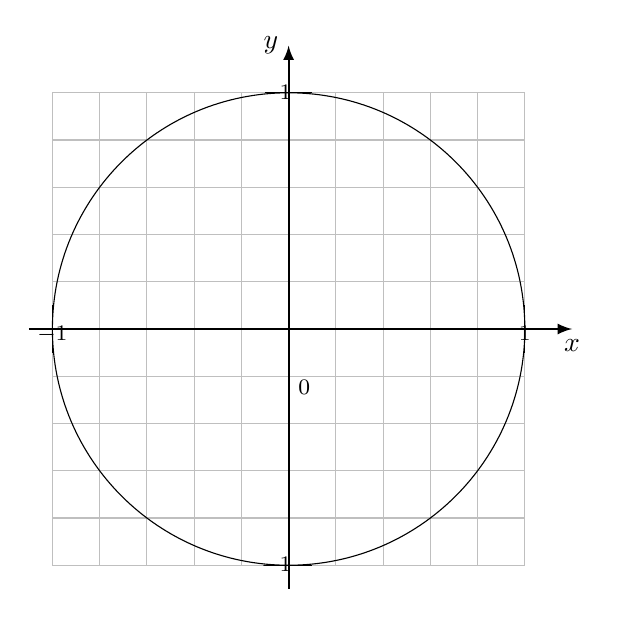
\begin{tikzpicture}[cross/.style={draw, cross out, minimum size=2*(#1-1pt), inner sep=0pt, outer sep=0pt}, x=10mm, y=10mm, 
        >=latex,   %Voreinstellung für Pfeilspitzen
        font= \footnotesize, scale=3]
        %Raster zeichnen
        \draw [color=gray!50]  [step=2mm] (-1,-1) grid (1,1);
        % Achsen zeichnen
        \draw[->,thick] (-1.1,0) -- (1.2,0) node[right, below] {\normalsize $x$};
        \draw[->,thick] (0,-1.1) -- (0,1.2) node[above, left] {\normalsize $y$};
        % Achsen beschriften
        \foreach \x in {-1,1} \draw (\x,-.1) -- (\x,.1) node[below=4pt] {$\x$};
        \foreach \y in {-1,1} \draw (-.1,\y) -- (.1,\y) node[left=4pt] {$\y$};
        % Besserer Ursprung
        \draw[color=black] (0pt,-7pt) node[right] {$0$};
        %Funktionen zeichnen:
        \clip(-1.1,-1.1) rectangle (1.1,1.1); %Bildbereich
        \draw circle [radius=1];
    \end{tikzpicture}
\end{figure}


%---------------------------------------------------------
\newpage
\question[6] % GZP 15 A7
Kreuze an, ob die folgenden Aussagen oder Gleichungen richtig oder falsch sind.\newline
\begin{table}[ht]
    \centering
    \begin{tabular}{l|c|c}
         & richtig & falsch\\\hline
        $\sin{(\alpha)}=\sin{(180^\circ-\alpha)}$ & & \\
        $\cos{(180^\circ-\beta)}=\cos{(180^\circ+\beta)}$ & & \\
        $\tan{(\alpha)}>0$ für $90^\circ<\alpha<180^\circ$ & & \\
        $\cos{(\alpha)}=\sin{(\alpha)}$ für $\alpha=\frac{\pi}{6}$ & & \\
        $\sin{(360^\circ-\beta)}=\sin{(180^\circ-\beta)}$ & & \\
        In einem Dreieck mit $\gamma=90^\circ$ gilt: $\sin{(\alpha)}=\cos{(90^\circ-\alpha)}$ & & \\
    \end{tabular}
\end{table}
\antwort{15}


%---------------------------------------------------------
\newpage
\question[3] % NW1 S188 A4
Welche der untenstehenden Winkel haben den gleichen Sinuswert?
\[\frac{\pi}{2},\qquad150^\circ, \qquad\frac{3\pi}{4}, \qquad90^\circ, \qquad\frac{\pi}{6}, \qquad45^\circ\]
Begründe mit Hilfe des Einheitskreises und ohne Verwendung des Taschenrechners.
\begin{figure}[ht]
    \begin{tikzpicture}[cross/.style={draw, cross out, minimum size=2*(#1-1pt), inner sep=0pt, outer sep=0pt}, x=10mm, y=10mm, 
        >=latex,   %Voreinstellung für Pfeilspitzen
        font= \footnotesize, scale=3]
        %Raster zeichnen
        % \draw [color=gray!50]  [step=7.5mm] (-1.3,-5.3) grid (14.8,5.8);
        % Achsen zeichnen
        \draw[->,thick] (-1.1,0) -- (1.2,0) node[right, below] {\normalsize $x$};
        \draw[->,thick] (0,-1.1) -- (0,1.2) node[above, left] {\normalsize $y$};
        % Achsen beschriften
        \foreach \x in {-1,1} \draw (\x,-.1) -- (\x,.1) node[below=4pt] {$\x$};
        \foreach \y in {-1,1} \draw (-.1,\y) -- (.1,\y) node[left=4pt] {$\y$};
        % Besserer Ursprung
        \draw[color=black] (0pt,-7pt) node[right] {$0$};
        %Funktionen zeichnen:
        \clip(-1.1,-1.1) rectangle (1.1,1.1); %Bildbereich
        \draw circle [radius=1];
    \end{tikzpicture}
\end{figure}


%---------------------------------------------------------
\newpage
\question[4] % Rhyn S6 A41
Ein Satellit befindet sich $100$km über dem Atlantik.\newline
\textit{Tipp: } Der Erdradius beträgt $6370$km.
\begin{parts} 
    \part Unter welchem Winkel ist der Rand der Erdkugel sichtbar?
\end{parts}
\vspace{5pt}
\antwort{10}
\begin{parts} 
    \setcounter{partno}{1}
    \part In welcher Entfernung ist der Rand der Erdkugel sichtbar?
\end{parts}
\vspace{5pt}
\antwort{10}


%---------------------------------------------------------
\newpage
\question[3] % GZP 15 A16
In einem rechtwinkligen Dreieck $ABC$ mit Hypothenuse $c$ sind die Seite $a=7$ und die Seitenhalbierende $s_a=4.5$ gegeben. Berechne die Länge der Winkelhalbierenden $w_\beta$.
\vspace{5pt}
\antwort{21}

\end{questions}
\end{document}